\noindent This section contains the experimental study surrounding our proposed algorithm. The aim of the experiments is to evaluate: 1. How the latency differs by different values of $k$, $l$ and $p$, and 2. How the setting of the parameters affects the amount of tuples getting stuck in the system, as well as discussing a possible solution to this shortcoming. As described earlier, due to the static generalization, there is no point in evaluating the information loss, since every tuple would be generalized in the same way, independent of the parameters, the information loss is constant. The only thing that can affect information loss is therefore the composition of the quasi-identifier, but since this is not a parameter that in reality can be chosen by the data publisher, we are not concerned with this scenario.
\\
\subsection{Data and experimental design}

\subsubsection{Data and experiment setup}

The \textit{adult} data set from the UCI Machine Learning repository was used as a starting point of these experiments \cite{dua2017}. Extraction of this data set was originally done by Barry Becker from the 1994 Census database. The distributions and unique values of this data set were used to create a data stream with the same characteristics of $n$ tuples. 

\begin{table}[H]
\centering
\begin{tabular}{llll}
\toprule
Data set characteristics & Attribute characteristics & Number of instances & Number of attributes \\ \hline
Multivariate             & Categorical, Integer      & 48842               & 14                   \\ \bottomrule
\end{tabular}
\caption{Characteristics of the \textit{adult} data set}
\label{datacharac}
\end{table}

\noindent For comparability, all evaluations were done with the quasi-identifier \textit{(age, educ, marital status)} with the generalization hierarchy levels described in table \ref{quasiGen}.

\begin{table}[H]
\centering
\begin{tabular}{cccc}
\toprule
Identifier & Generalization Level & Number of classes \\ 
\midrule
Age & 2 & 10 \\
Education & 2 & 3 \\
Marital Status & 1 & 2 \\ \midrule
Sensitive attribute \\ (not part of QID) & - & 10 \\
\bottomrule
\end{tabular}
\caption{Quasi-Identifier generalization}
\label{quasiGen}
\end{table}

\noindent The experiments were conducted on Apache Flink (version 1.3) in "mini cluster"-mode on a mid 2015 Apple Macbook Pro with 2,2 GHz Intel Core i7 processor and 16GB 1600 MHz DDR3 RAM. 

\subsubsection{Parameters}
The parameters subject to variation in the experiments were the following:
\begin{itemize}
\renewcommand{\labelitemi}{}
\item \textbf{k} - The k-anonymity constraint.
\item \textbf{l} - The l-diversity constraint.
\item \textbf{n} - The stream length, i.e. the number of tuples in the stream.
\item \textbf{p} - The parallelism, i.e. the number of parallel processes in Apache Flink. 
\end{itemize}

\subsection{Experiments and results}

\subsubsection{Overall speed}

This experiment serves to show the overall speed of the anonymization process for different parameters. This will later serve as an indicator of algorithm efficiency, since a data stream would possibly never ending in practice.

\begin{figure}[H]
    \centering
    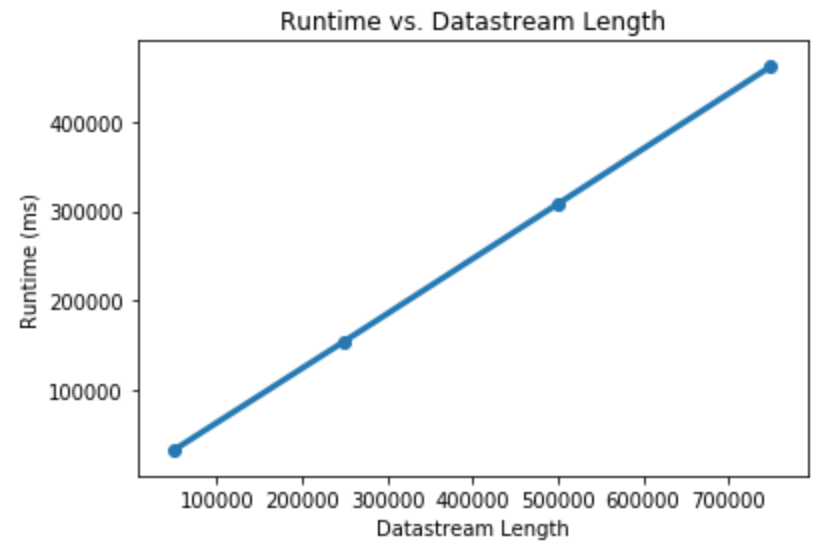
\includegraphics[scale=0.8]{Images/runtime.png}
    \caption{Run time (ms) for data streams of length \textit{n = 50 000, 250 000, 500 000 and 750 000}} $(k=40, l=5, p=10)$.
    \label{fig:runtime}
\end{figure}

\noindent As can be seen from figure \ref{fig:runtime}, the overall running time increases linearly with $n$. 


\begin{figure}[H]
    \centering
    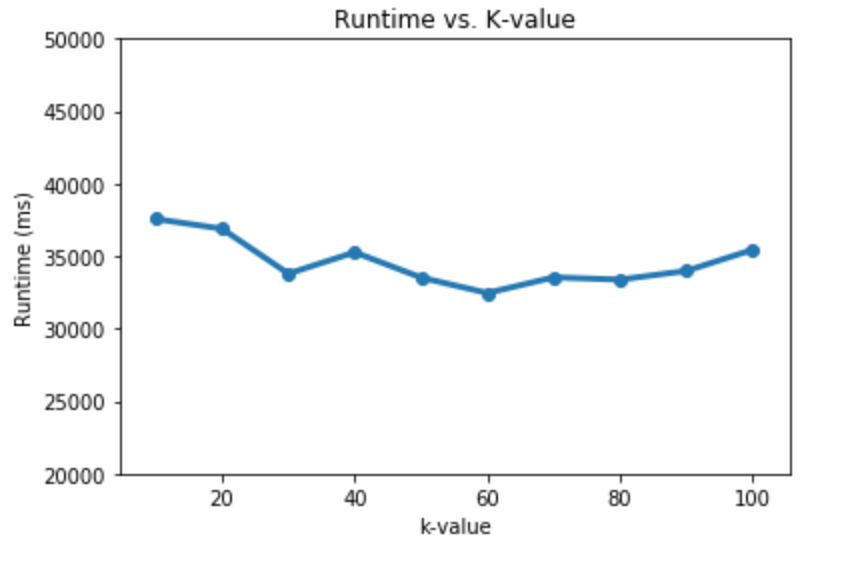
\includegraphics[scale=0.8]{Images/runtimekvals.png}
    \caption{Run time (ms) for values of  \textit{10 \leq k \leq 100}} and $n=50 000, l=5, p=10$.
    \label{fig:runtimekvals}
\end{figure}

\noindent As can be seen from figure \ref{fig:runtimekvals}, the overall running time is more or less constant for different values of $k$. 

\begin{figure}[H]
    \centering
    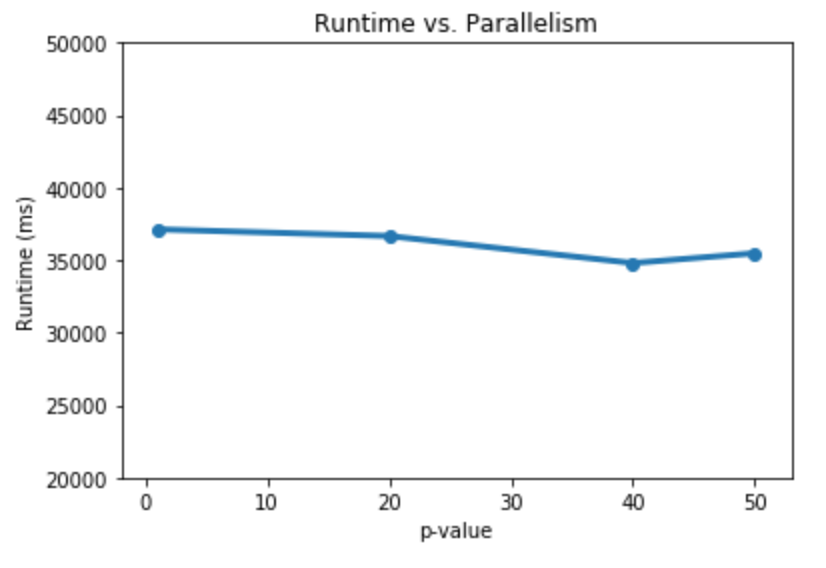
\includegraphics[scale=0.7]{Images/runtimepvals.png}
    \caption{Run time (ms) for values of  \textit{p = 1, 10, 20, 30, 40, 50}} and $n=50 000, l=5, k=40$.
    \label{fig:runtimepvals}
\end{figure}

\noindent As can be seen from figure \ref{fig:runtimepvals}, the overall running time is more or less constant for different values of $p$. 


\subsubsection{Tuple Delay}
For each tuple processed in accordance to the algorithm in section 3.B, a delay is induced. While some delay is inescapable, too much delay might render the data to be inaccurate or irrelevant by the time it is omitted. In the first part of the experiments, we aim to establish a better understanding of how the delay varies depending on the different variables \textit{k, l} and \textit{p}. The tuple delay is measured through adding an injection timestamp to each AdultData-object upon tuple arrival, and adding a processing timestamp just before the object is emitted. In these experiments the stream length \textit{n} was fixed to \textit{n = 50000}.\\
\\
\textbf{K-anonynymity} \\
%$20 \leq k \leq 80$ with \textit{l = 5} and \textit{p = 10}. 
\begin{figure}[H]
    \centering
    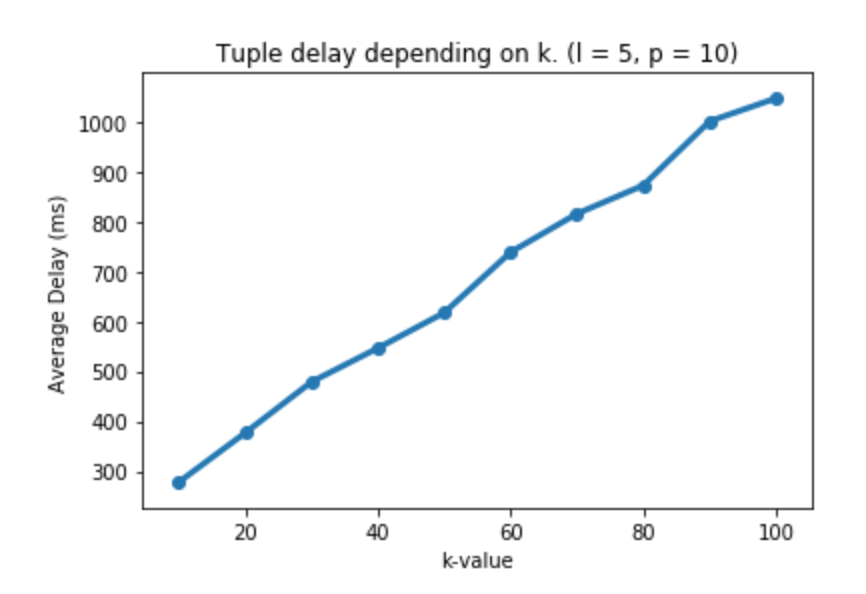
\includegraphics[scale=0.7]{Images/k-values.png}
    \caption{Average tuple delay depending on k, \textit{(l = 5, p = 10)}}
    \label{fig:kvalues}
\end{figure}

\noindent As can be seen from figure \ref{fig:kvalues}, the average delay of the tuples increases linearly with $k$.
\newpage
\noindent \textbf{L-diversity} \\
%$1 \leq l \leq 10$ with \textit{k = 40}, \textit{p = 10}

\begin{figure}[H]
    \centering
    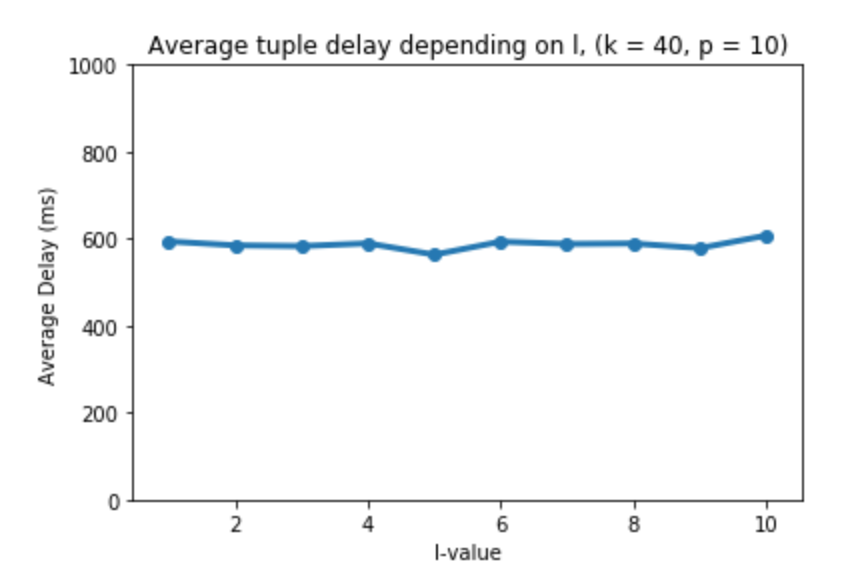
\includegraphics[scale=0.8]{Images/l-values.png}
    \caption{Average tuple delay depending on l, \textit{(k = 40, p = 10)}}
    \label{fig:lvalues}
\end{figure}

\noindent As can be seen from figure \ref{fig:lvalues}, the average delay was more or less constant for different values $l$.\\
\\
\textbf{Parallelism} \\%($5 \leq p \leq 50$ with \textit{k = 40} and \textit{l = 5}. )

\begin{figure}[H]
    \centering
    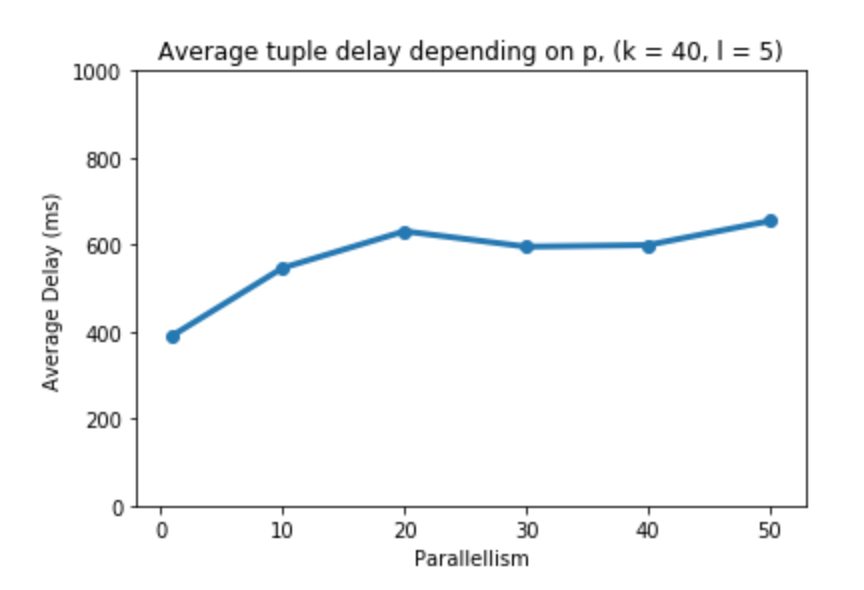
\includegraphics[scale=0.8]{Images/p-values.png}
    \caption{Average tuple delay depending on p, \textit{(k = 40, l = 5)}}
    \label{fig:pvalues}
\end{figure}

\noindent As can be seen from figure \ref{fig:lvalues}, the experience could show no trivial correlation between the average tuple delay and the number of parallel processes.  $l$.

\subsubsection{Stuck Tuples}

\begin{figure}[H]
    \centering
    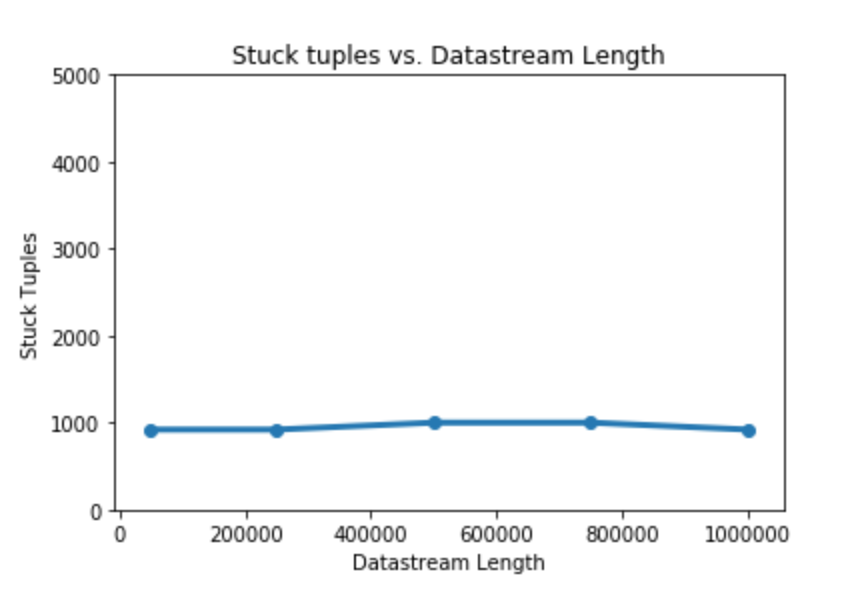
\includegraphics[scale=0.8]{Images/numbertuples.png}
    \caption{Number of stuck tuples for data streams of length \textit{n = 50 000, 250 000, 500 000, 750 000 and 1 000 000}. }
    \label{fig:stucknum}
\end{figure}

\begin{figure}[H]
    \centering
    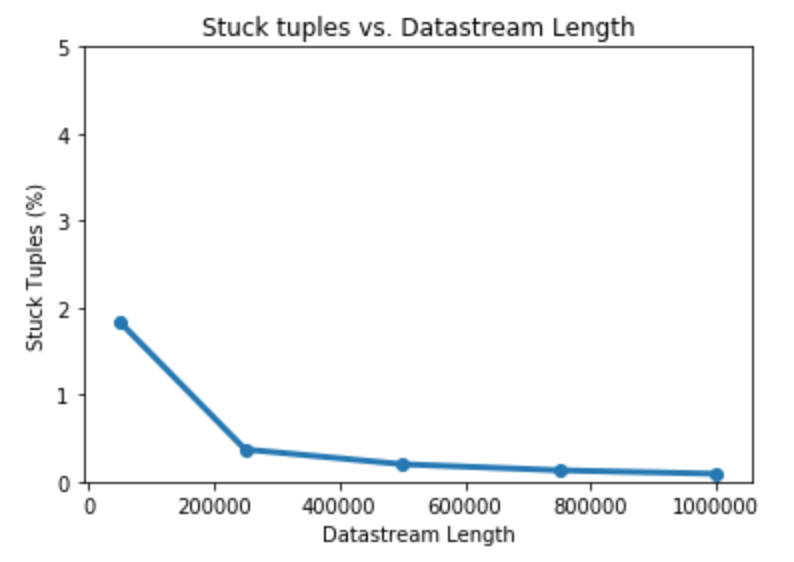
\includegraphics[scale=0.8]{Images/percenttuples.png}
    \caption{Stuck tuples as a percentage of total data stream length, for data streams of length \textit{n = 50, 250, 500, 750 and 1000 $*$ $10^3$} .}
    \label{fig:stuckpercent}
\end{figure}

\noindent As can be seen from figure \ref{fig:stucknum} and \ref{fig:stuckpercent}, it could be shown that the number of stuck tuples was constant for streams of lengths up to \textit{n = 1 000 000}. 


\begin{figure}[H]
    \centering
    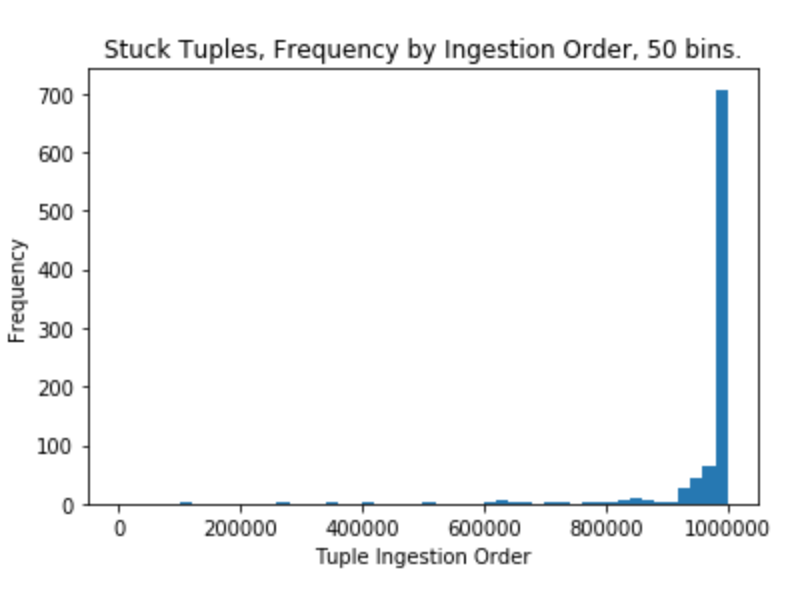
\includegraphics[scale=0.8]{Images/tupledistribution.png}
    \caption{Stuck tuples, frequency by ingestion order for a data stream of length \textit{n = 100000}. }
    \label{fig:stuckdist}
\end{figure}

\noindent As can be seen from figure \ref{fig:stuckdist}, it could be shown that the stuck tuples were in majority a part of the last tuples according to ingestion order. (reformulate??) 

\subsection{Discussion}

\subsubsection{Runtime and Tuple Delay} % Commenting on the results of n,K,L,P experiments. 

First of all, the runtime was expectedly linear to the data stream length, which helps us draw the conclusion that the algorithm probably not will be neither more or less efficient for infinitely long data streams. \\
As it was to be expected, the average delay of the tuples increases with an increase of $k$, as shown in fig \ref{fig:kvalues}. As the window for each $QID$ needs more tuples to reach K-anonymity and thereby released, the result is longer relay for the tuples already in that window. In comparison, the runtime evaluation of different values of $k$ in fig. \ref{fig:runtimekvals} showed that despite these delays, the algorithm in itself still finishes with constant efficiency independent of the size of $k$. \\
However, it is hard to draw conclusions regarding the tuple delay variation depending on $l$. In our experiments, the runtime appears to be constant for any $1 \leq l \leq 10 $, where 10 is the number of different sensitive classes in our data and hence the largest possible diversity among any group of tuples. Since this is a relatively small value, for example in comparison to $k$, it can not be excluded that the runtime may vary for larger values of $l$. \\
% Probably remove but not sure: This result differs from most previous approaches which use k-anonymity on batches of data. Assumably, this is due to that large batches of data and faster, that is why other researchers find decreasing latencies for larger k. for us it is the other way around. however anonymizing large batches, has the shortcoming that there might be outliers and therefore the generalization needs to be strong in order to get all tuples on one level, which leads to a large information loss
As seen in fig. \ref{fig:runtimepvals} and fig. \ref{fig:pvalues}, it could not be found that the method benefited from parallelization in terms of either total efficiency or tuple delay. A possible explanation could be that in the current setup, the overhead of running multiple processes is higher than the possible benefits of the parallelization, thus preventing real advantage. It is possible that parallelization will be more beneficial as the number of possible $QID$ generalizations increase. 

\subsubsection{Stuck Tuples} % Commenting on the stuck tuples experiments and our approach in general 
The experiments could show that the number of stuck tuples remained constant for any tested data stream length. This is an expected outcome. As mentioned in section \ref{sect:algorithm} the amount of stuck tuples has an upper bound induced by the number of unique possible combinations of the generalized quasi-identifier. Furthermore, the distribution of fig. \ref{fig:stuckdist} show that the tuples still in the pipeline was predominantly tuples which were inserted during the last 10\% of the data stream lifetime. While expected, these results verify that the logic behind the approach of keying tuples by $QID$ is actually working in practice. However, it must be pointed out that the upper bound of stuck tuples will become significantly bigger with a more complex $QID$, and that depending on data distribution a significant amount of tuples may still become stuck indefinitely in some implementations. 

\subsubsection{The keying by $QID$-approach} % Suggesting future experiments (especially regarding our approach)
As mentioned in \ref{sect:algorithm}, many current approaches of applying \textit{k}-anonymity on streamed data induce an information loss that increases linearly with \textit{k}. Through these evaluations, we could show that the approach of keying by $QID$ with a weak, static generalization introduces a comparably small information loss, at the price of an introduced tuple delay. While the mentioned approach may reduce information loss, there still remains tuples in the pipeline considered as stuck or very delayed in the current form of the approach. As a possible solution, we would like to suggest the possibility to continuously collecting, applying \textit{k}-anonymizing and releasing tuples which are considered as stuck according to a certain constraint. Such a constraint could be either expressed as time delay or order delay. As the percentage of stuck tuples showed to be very low, the potential information loss in total remains low. 

% Notes MM:
% I guess we could reason in the report that through our method, we can apply % a weak generalization, thus reducing information loss. Then, the stuck % % % tuples (in our case ca 15% of the total number of tuples) will be 
% anonymized with the algorithm.




